\documentclass[12pt, a4paper]{article}
\usepackage{header}

% \numberwithin{equation}{section}

\title{\textbf{\sffamily{Segon Lliurament de Càlcul de Diverses Variables i Optimització}}}
\author{\textsf{Arnau Mas}}
\date{\textsf{8 de Gener de 2018}}

\begin{document}
\selectlanguage{catalan}
\maketitle

\section*{Problema 1} \label{sec:problema 1}
Sen's demana de resoldre una equació diferencial en derivades parcials fent servir un canvi de coordenades. L'equació en qüèstió és 
\begin{equation}
  f_{xx}(x,y,z) - f_{yy}(x,y,z) + f_{zz}(x,y,z) - 2f_{xz}(x,y,z) = (y + z)(x + z) \label{eq:eq diferencial}.
\end{equation}
La solució \( f \colon \R^3 \to \R \) suposarem que és una funció de classe \( C^2(\R^3) \). El canvi que sen's proposa ve donat per
\begin{equation}
	\begin{aligned}
		\Psi \colon \R^3 & \to \R^3 \\  
		(x,y,z) & \mapsto (x+y, y+z, z+x) .
	\end{aligned} 
	\label{eq:canvi de variables}
\end{equation}
Denotem les components de \( \Psi \) per \( u \), \( v \) i \( w \). És clar que \( \Psi \) és una bijecció lineal i per tant un difeomorfisme. Definim \( g = f \circ \Psi^{-1} \). D'aquesta manera es compleix \( f = g \circ \Psi \) i podem, fent servir la regla de la cadena, reescriure l'equació diferencial en termes de les noves coordenades. 
\begin{equation}
	\begin{aligned}
  	f_x &= g_u u_x + g_v v_x + g_w w_x = g_u + g_w \\
  	f_y &= g_u u_y + g_v v_y + g_w w_y = g_u + g_v \\
  	f_z &= g_u u_z + g_v v_z + g_w w_z = g_v + g_w. 
	\end{aligned}
	\label{eq:primeres derivades}
\end{equation}
Tornem a derivar:
\begin{align*}
	f_{xx} &= g_{uu}u_x + g_{uv}v_x + g_{uw}w_x + g_{wu}u_x + g_{wv}v_x + g_{ww}w_x  \\
				 &= g_{uu} + 2g_{uw} + g_{ww} \\
	f_{yy} &= g_{uu}u_x + g_{uv}v_x + g_{uw}w_x + g_{vu}u_x + g_{vv}v_x + g_{vw}w_x  \\
				 &= g_{uu} + 2g_{uv} + g_{vv} \\
	f_{zz} &= g_{vu}u_z + g_{vv}v_z + g_{vw}w_z + g_{wu}u_z + g_{wv}v_z + g_{ww}w_z  \\
				 &= g_{vv} + 2g_{vw} + g_{ww} \\
	f_{xz} &= g_{uu}u_z + g_{uv}v_z + g_{uw}w_z + g_{wu}u_z + g_{wv}v_z + g_{ww}w_z  \\
				 &= g_{uv} + g_{uw} + g_{wv} + g_{ww}. \\
\end{align*}
I per tant 
\begin{equation}
  f_{xx} + f_{yy} + f_{zz} - 2f_{xz} = -4g_{uv}. 
\end{equation}
Així doncs, l'equació diferencial en les noves coordenades és 
\begin{equation}
  g_{uv}(u,v,w) = -\dfrac{1}{4}vw. \label{eq:nova eq diferencial}
\end{equation}
En aquesta forma, podem solucionar \ref{eq:nova eq diferencial} de forma immediata per integració:
\begin{equation}
  g(u,v,w) = -\dfrac{1}{8}uwv^2 + A(v,w) + B(u,w), \label{eq:solucio general}
\end{equation}
on \( A \) i \( B \) són funcions arbitràries que compleixen \( A_u = B_v = 0 \). I en les coordenades originals, la solució és
\begin{equation}
  f(x,y,z) = -\dfrac{1}{8}(x+y)(x+z)(y+z)^2 + A(y+z,x+z) + B(x+y,x+z).
\end{equation}

Un cop tenim la solució general podem trobar la solució particular que sen's demana aplicant les condicions inicials. Tenim que, en el pla \( x+y = 0 \) es compleix \( f_y + f_z - f_x = 0 \). Fent servir \ref{eq:primeres derivades} veiem que aquesta condició, traduïda a les noves coordenades, és equivalent a \( g_v = 0 \) en els punts del pla \( u = 0 \). A partir de \ref{eq:solucio general} tenim que \( g_u(u,v,w) = -\frac{1}{4}uvw + A_v(v,w) \). Per tant, per tots els punts que compleixen \( u = 0 \) tenim que \( A_v(v,w) = 0 \), i per tant que \( A \) només depèn de \( w \).

Sabem també que \( f = 0 \) restringida als punts del pla \( x = 0 \). Traduït a les noves coordenades, \( g = 0 \) als punts del pla \( v = u + w \). Per tant, per tot \( u,w \in \R \) es compleix
\begin{equation*}
  -\dfrac{1}{8}uw(u+w)^2 + A(w) + B(u,w) = 0,
\end{equation*}
i per tant la solució que busquem és \( g(u,v,w) = \frac{1}{8}uw\left((u+w)^2 - v^2\right) \).

Per veure que és única considerem dues potencials solucions, \( g_1 \) i \( g_2 \) i la seva diferència \( h = g_1 -g_2 \). Per linealitat tenim que \( h \) compleix \( h_{uv} = 0 \). Això ens dóna que \( h = A + B	\) amb \( A_u = B_v = 0 \). La funció \( h \) clarament també compleix les condicions inicials que compleixen \( g_1 \) i \( g_2 \). Així tenim, que en el pla \( u = 0 \), \( h_v(0,v,w) = A_v(v,w) = 0 \), per tant que \( A \) només depèn de \( w \). Per la segona condició, sabem que \( h \) és nul·la restringida als punts que compleixen \( v = u + w \). És a dir \( h(u,u+w,w) = 0 \) per tot \( u,w \in \R \). Però com que \( h \) no depèn de \( v \) concloem que \( h \) és idènticament zero i per tant \( g_1 = g_2 \), com volíem.

\section*{Problema 2}



\section*{Problema 3}
Sen's demana calcular el volum de la intersecció entre l'interior de l'el·lipsoide d'equació \[ \dfrac{x^2}{a^2} + \dfrac{y^2}{b^2} + \dfrac{z^2}{c^2} = 1 \] i el semiespai donat per \[ Ax + By + Cz \leq D . \] Observem que podem fer un canvi de coordenades per a reduir al problema al càlcul del volum d'un casquet esfèric. Concretament el canvi que fem servir és el definit per 
\begin{align*}
	H \colon \R^3 & \to \R^3 \\
	(x,y,z) & \mapsto \left(\dfrac{x}{a},\dfrac{y}{b},\dfrac{z}{c}\right).
\end{align*}
Si denotem les noves coordenades per \( (u,v,w) \) tenim que ara l'el·lipsoide té equació \( u^2 + v^2 + w^2 = 1 \) i ja no és un el·lipsoide sino que és una esfera. L'equació del semiespai es transforma en \( Aau + Bbu + Ccw \leq D \). És clar que \( H \) és una bijecció lineal i per tant un difeomorfisme. Calcular-ne la inversa és immediat i tenim que el jacobiá de \( H^{-1} \) és \( J_{H^{-1}}=abc \). Així doncs, pel teorema del canvi de variable tenim que si denotem per \( A \) el conjunt del qual en volem calcular el volum:
\begin{equation}
	m(A) = \int_A \mathbf{1}_A = \int_{H(A)} \mathbf{1}_{H(A)} \abs{J_{H^{-1}}} = \abs{abc} \int_{H(A)} \mathbf{1}_{H(A)} = \abs{abc}m(H(A)). \label{eq:canvi de variables per simplificar}
\end{equation}
Podem suposar, sense pèrdua de generalitat, que \( a \), \( b \) i \( c \) són reals positius.

La regió de la qual hem de calcular el volum ara, \( H(A) \) és un casquet esfèric. El volum, \( V \), d'un casquet esfèric d'una esfera de radi \( r \) està donat per
\begin{equation}
	V = \dfrac{\pi h^2}{3}(3r - h), \label{eq:volum d'un casquet}
\end{equation}
on \( h \) és l'alçada del casquet. En el nostre cas, \( r = 1 \). Ens serà útil reescriure \ref{eq:volum d'un casquet} en funció de la distància entre el pla que defineix el casquet i l'origen. La distància, \( d \), entre el pla ---després del canvi de coordenades---	i l'origen ve donada per 
\begin{equation}
	d = \dfrac{D}{\sqrt{A^2a^2 + B^2b^2 + C^2c^2}}. \label{eq:definicio de d}
\end{equation}
Tal i com la definim, \( d \) pot ser negativa o positiva en funció del signe de \( D \). Això distingeix si el pla es troba per sota de l'origen, \( d < 0 \), o per sobre, \( d > 0 \). Tenim que \( h \) serà més petita que \( 1 \) quan \( d < 0 \), i de fet \( h - d = 1 \). Així doncs, substituïnt a \ref{eq:volum d'un casquet} obtenim
\begin{equation}
	m(H(A)) = \dfrac{\pi(1 + d)^2}{3}(2 - d) = \dfrac{\pi}{3}\left(2 + 3d - d^3\right).
\end{equation}
I finalment, recuperant \ref{eq:canvi de variables per simplificar} tenim
\begin{equation}
	m(A) = \dfrac{\pi}{3}abc (2 + 3d - d^3)
\end{equation}
amb \( d \) definida com a \ref{eq:definicio de d}. Ometem el valor absolut ja que, tal i com hem indicat abans, podem suposar sense pèrdua de generalitat que \( a, b, c \geq 0 \).



\section*{Problema 4} \label{sec:problema 4} 
Observem que en coordenades cartesianes, podem parametritzar la cardioide que té per equació \( r = 1 + \cos{\varphi} \) com
\begin{equation}
  \begin{aligned}
    x(\varphi) &= (1 + \cos{\varphi})\cos{\varphi} \\
    y(\varphi) &= (1 + \cos{\varphi})\sin{\varphi}
  \end{aligned}
	\label{eq:parametrització cardioide de revolució}
\end{equation}

amb \( \varphi \in (0, 2\pi) \). Per a parametritzar la superfície \( S \) que resulta quan la cardioide gira al voltant de l'eix \( x \) introduïm un nou paràmetre \( \theta \), que representarà l'angle de rotació. Com que la cardioide és simètrica, només ens cal la secció que correspon a \( \varphi \in (0, \pi) \). Podem parametritzar \( S \) mitjançant una funció \( H\colon (0,\pi) \times (0,2\pi) \to \R^3 \) amb 
\begin{equation}
  H(\varphi,\theta) = ((1+\cos{\varphi})\cos{\varphi}, (1+\cos{\varphi})\sin{\varphi}\cos{\theta}, (1+\cos{\varphi})\sin{\varphi}\sin{\theta}). \label{eq:cardioide de revolució}
\end{equation}
És clar que \( H \) és un difeomorfisme en la seva imatge, i per tant defineix \( S \) com una varietat regular. Per ser rigurosos, amb aquesta parametrització ens deixem tot un arc del cardioide, que són tots els punts amb \( \theta = 0 \). Ara bé, a l'hora d'integrar no cal que ens preocupem ja que aquest conjunt té àrea nul·la. Si prenem com a domini de la parametrització \( [0,\pi] \times [0,2\pi] \)	obtenim tota la superfície.

\begin{figure}[htb]
  \centering
  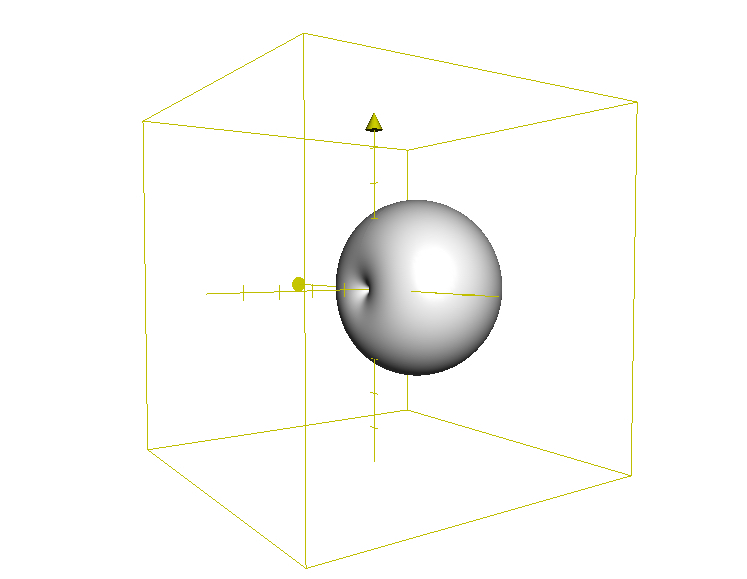
\includegraphics[scale = 0.4]{cardioide.jpg}
 	\caption{Resultat de la parametrització donada per \ref{eq:parametrització cardioide de revolució}} 
\end{figure}

Per calcular l'àrea d'una superfície donada per una parametrització hem de trobar l'element d'àrea i integrar-lo en el domini de la parametrització. Ara bé, podem aprofitar que \( S \) no és una varietat qualsevol, sino que és una superfície de revolució. En general, l'element d'àrea de la superfície de revolució que resulta de rotar l'arc \( \gamma(\varphi) = (x(\varphi), y(\varphi), 0) \) al voltant de l'eix \( x \) és 
\begin{equation}
  dA = y(\varphi)\norm{\dot{\gamma}(\varphi)} d\varphi \, d\theta = y(\varphi)\sqrt{\dot{x}(\varphi)^2 + \dot{y}(\varphi)^2} d\varphi \, d\theta. 
\end{equation}
A més, l'arc \( \gamma \) està donat en coordenades polars, així que és de la forma \( \gamma(\varphi) = r(\varphi) (\cos{\varphi}, \sin{\varphi}, 0) \) i per tant \( \norm{\dot{\gamma}(\varphi)} = \sqrt{r(\varphi)^2 + \dot{r}(\varphi)^2} \). Així doncs, l'àrea de \( S \), és a dir la mesura 2-dimensional de \( S \) és
\begin{align*}
 	m_2(S) &= \int_0^{2\pi} \! \int_0^\pi (1+\cos{\varphi})\sin{\varphi} \sqrt{(1+\cos{\varphi})^2 + \sin{\varphi}^2} \, d\varphi \, d\theta \\	
				 &= \int_0^{2\pi} \! \int_0^\pi (1+\cos{\varphi})\sin{\varphi} \sqrt{2(1 + \cos{\varphi})} \, d\varphi \, d\theta \\
				 &= -2\pi\sqrt{2} \int_0^\pi (1 + \cos{\varphi})^{3/2} \sin{\varphi} \, d\varphi \\ 
				 &= \left[-\dfrac{4\pi\sqrt{2}}{5} (1 + \cos{\varphi})^{5/2}\right]_0^\pi = \dfrac{32\pi}{5} 
\end{align*}

Observem que el punt \( \left(\frac{1}{2}(1+\sqrt{2}),\frac{1}{2}(1+\sqrt{2})\right) \) és precisament la imatge de \( \varphi = \pi/4 \) al cardioide. Així doncs, l'òrbita d'aquest punt quan fem girar el cardioide per generar \( S \) és el conjunt de punts de la forma \( H(\pi/4, \theta) \) amb \( \theta \in [0, 2\pi] \). Si volem calcular el pla tangent a \( S \) en qualsevol d'aquests punts, cal que avaluem les derivades parcials de \( H \) en aquests punts. Tenim
\begin{equation}
	\dfrac{\partial}{\partial \varphi}(\theta,\varphi) = \partial_{\varphi}H(\varphi, \theta) = \begin{bmatrix}
    -\sin{\varphi}(1 + 2\cos{\varphi}) \\
    (\cos{\varphi} + \cos{\varphi}^2 - \sin{\varphi}^2)\sin{\theta} \\
    (\cos{\varphi} + \cos{\varphi}^2 - \sin{\varphi}^2)\cos{\theta} 
  \end{bmatrix} \label{eq:parcial 1}
\end{equation}
i
\begin{equation}
	\dfrac{\partial}{\partial \theta}(\varphi, \theta) = \partial_{\theta}H(\varphi, \theta) = (1 + \cos{\varphi}) \begin{bmatrix}
    0 \\
    \sin{\varphi}\cos{\theta} \\
    -\sin{\varphi}\sin{\theta}
  \end{bmatrix} . \label{eq:parcial 2}
\end{equation}

El pla tangent a una superfície regular donada per una parametrització està generat per les derivades parcials de la parametrització. En els punts de l'òrbita que estem considerant ---és a dir, els punts amb \( \varphi = \pi/4 \)--- el pla tangent en funció de l'angle \( \theta \), \( \pi(\theta) \), està donat, com a subvarietat afí per
\begin{align*}
  \pi(\theta) &= H(\pi/4, \theta) + \left\langle \dfrac{\partial}{\partial \varphi}(\pi/4, \theta), \dfrac{\partial}{\partial \theta}(\pi/4, \theta) \right\rangle \\ 
							&= \dfrac{1+\sqrt{2}}{2} (1, \sin{\theta}, \cos{\theta}) \\
							& \quad +{} \left\langle \left(-\left(1+\sqrt{2}\right), \sin{\theta}, \cos{\theta}\right), (0, \cos{\theta}, -\sin{\theta}) \right\rangle \yestag \label{eq:multiplicar per escalars} .
\end{align*}
Al pas \ref{eq:multiplicar per escalars} s'ha dividit la parcial respecte de \( \theta \) per \( \frac{1}{\sqrt{2}}(1 + \sqrt{2}) \) i la parcial respecte de \( \varphi \) s'ha multiplicat per \( \sqrt{2} \). Fer això no afecta l'àlgebra lineal i alleugereix la notació.

Si volem donar una equació pel pla, observem que el vector \[ u = \left(1, \left(1+\sqrt{2}\right)\sin{\theta},  \left(1+\sqrt{2}\right)\cos{\theta}\right) \] és de l'ortogonal de \( \pi(\theta) \). Per tant, l'equació del pla tangent és:
\begin{equation*}
	\inn{u}{(x,y,z) - H(\pi/4, \theta)}.
\end{equation*}
Més en detall:
\begin{equation}
	x +\left(\left(1 + \sqrt{2}\right)\sin{\theta}\right)\! y +\left(\left(1 + \sqrt{2}\right)\cos{\theta}\right)\! z = \dfrac{4 + 3\sqrt{2}}{2}. 
\end{equation}


\end{document}
